%% === Preamble ============================================
\documentclass[
  %parskip = half,
  %draft = false,
  %twoside = false,
  11pt
]{article}
\usepackage[utf8]{inputenc}
%\usepackage[ngerman]{babel}
\usepackage{csquotes}

%% --- PDF setup -------------------------------------------
\usepackage[
  %pdftex,
  pdfpagelabels=false,
  bookmarksopenlevel=chapter
]{hyperref}
\hypersetup{
  pdftitle = {Linkspop und Rechtspop}
  pdfauthor = {Werner Krause},
  bookmarksnumbered = true,
  bookmarksopen = false,
  colorlinks = true,
  linkcolor = blue,
  citecolor = blue,
  urlcolor = blue
}

\usepackage[titletoc]{appendix}
\usepackage{pdfpages}

%% --- Page setup ------------------------------------------
\usepackage{scrpage2}                             %% Headers
  \pagestyle{scrheadings}
\usepackage[hang]{footmisc}
\usepackage{lineno}
\usepackage{setspace}
\usepackage{blindtext}
\clubpenalty = 10000                           % no orphants
\widowpenalty = 10000 \displaywidowpenalty = 10000 % no widows
\usepackage[left=1in,right=1in,top=1in,bottom=1in]{geometry}

%% --- Tables and floats -----------------------------------
\usepackage{booktabs}
\usepackage{multirow}
\usepackage{caption}
\usepackage{subcaption}
\usepackage{afterpage}
\usepackage{lscape}
\usepackage{dcolumn}

%% --- library ---------------------------------------------
%\usepackage[
%    backend=biber,
%    style=authoryear-icomp,
%    sortlocale=de_DE_phonebook,
%    natbib=true,
%    url=false,
%    doi=false,
%   isbn=false,
%    eprint=false
%]{biblatex}
%  \bibliography{PopulismLeviathan}
\usepackage{natbib}
%% --- Symbols, graphics, and blindtext --------------------
\usepackage{amsmath}
\usepackage{amssymb}
\usepackage{amsbsy}
\usepackage{amsthm}

\usepackage{tikz}
  \usetikzlibrary{positioning,backgrounds}

\usepackage{graphicx}

\usepackage{xcolor}
\definecolor{grey65}{cmyk}{0,0,0,0.3490}
\definecolor{grey20}{cmyk}{0,0,0,.2000}

%% --- Author ----------------------------------------------
\title{Repro Case Study: GovElec}
\author{Werner Krause\thanks{werner.krause@wzb.eu}, Dag Tanneberg\thanks{dag.tanneberg@wzb.eu}}
\date{\today}

\begin{document}
%\pagenumbering{roman}
%\linenumbers
\maketitle

\thispagestyle{empty}

\clearpage
\setcounter{page}{1}
%\doublespacing
\onehalfspacing

\section{Introduction}
\textit{Comment: Please answer these introductory questions for your case study in a few sentences.}

\noindent
\textit{1) Who are you and what is your research field? Include your name, affiliation, discipline, and the background or context of your overall research that is necessary specifically to introduce your specific case study.}

\noindent
\textit{2) Define what the term ``reproducibility'' means to you generally and/or in the particular context of your case study.}

\section{Workflow diagram}
\textit{Comment: The core of your case study is a diagrammatic workflow sketch, which depicts your the entire pipeline of your workflow. Think of this like a circuit diagram: boxes represent steps, tools, or other disjoint components, and arrows show how outputs of particular steps feed as inputs to others. This diagram will be complemented by a textual narrative.}

\noindent
\textit{We recommend the site draw.io for creating this diagram, or you are also welcome to sketch this by hand. While creating your diagram, be sure to consider: specialized tools and where they enter your workflow, the ``state'' of the data at each stage, collaborators, version control repos, products produced at various stages (graphics, summaries, etc), databases, whitepapers, customers.}

\noindent
\textit{Each of the two example case studies include a workflow diagram you can also use for guidance. Please save your diagram alongside this completed case study template.}

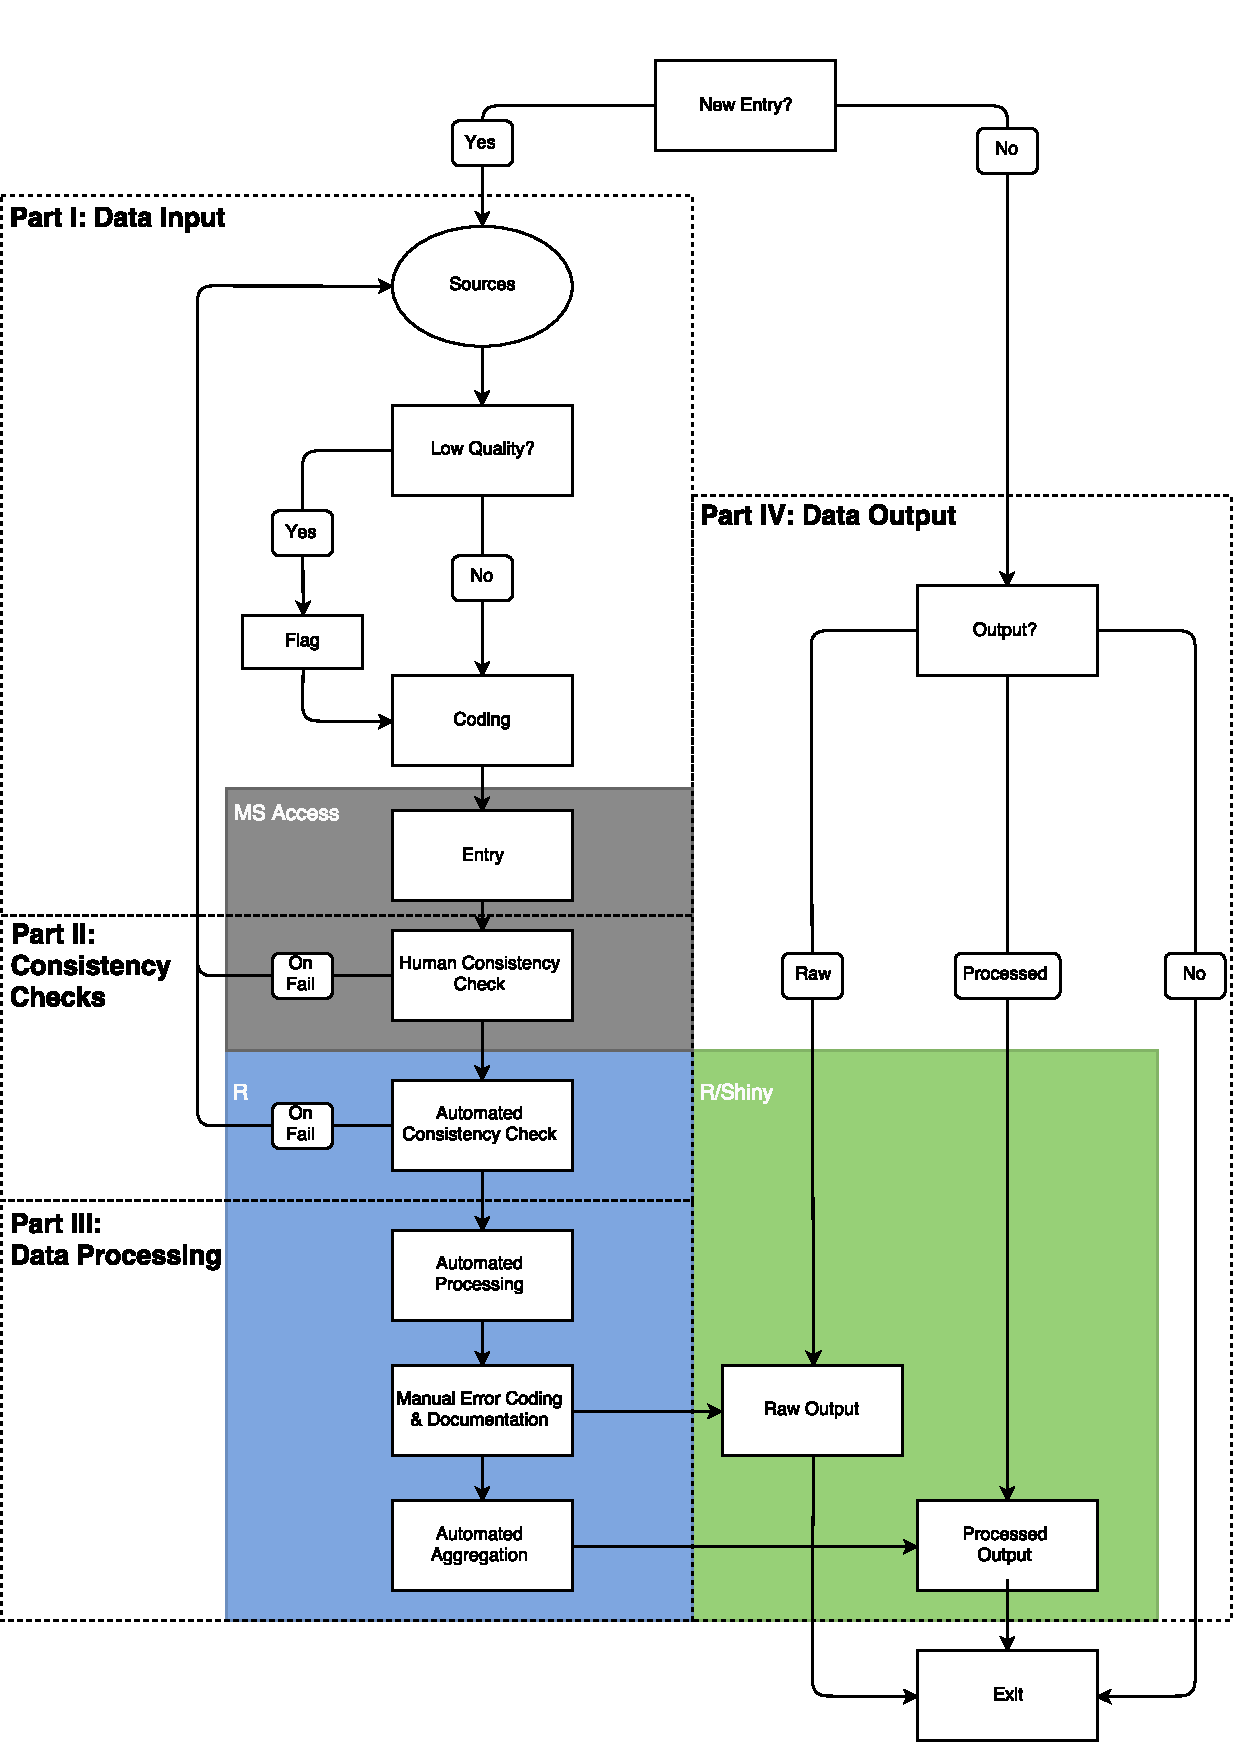
\includepdf{GovElec_Workflow_May2k16.pdf}

\section{Workflow narrative}

\textit{Comment: Referring to your diagram, describe your workflow for this specific project, from soup to nuts. Imagine walking a friend or a colleague through the basic steps, paying particular attention to links between steps. Don't forget to include ``messy parts'', loops, aborted efforts, and failures.}

\noindent
\textit{It may be helpful to consider the following questions, where interesting, applicable, and non-obvious from context. For each part of your workflow:}

\noindent
\textit{Frequency: How often does the step happen and how long does it take?}

\noindent
\textit{Who: Which members of your team participate (or not)?}

\noindent
\textit{Manual/Automated: Is the step automated or does it involve human intervention (if so, is it recorded)?}

\noindent
\textit{Tools: Which software or online tools are used in the step? How are they used?}

\noindent
\textit{In addition to detailing the steps of the workflow, you may wish to consider the following questions about the workflow as a whole:}

\noindent
\textit{Data: Is your raw data online?}

\textit{Is it citeable?}

\textit{Does the license allow external researchers to publish a replication/confirmation of your published work?}

\noindent
\textit{Software: Is the software online?}

\textit{Is there documentation?}

\textit{Are there tests?}

\textit{Are there example input files alongside the code?}

\noindent
\textit{Processing: Is your data processing workflow online?}

\textit{Are the scripts documented?}

\textit{Would an external researcher know what order to run them in?}

\textit{Would they know what parameters to use?}

\vspace*{1cm}

\noindent
Our workflow can be distinguished into four separate steps which can be fulfilled independently of each other. Apart from the single steps of the workflow, the colored areas document the software and tools that is used in each step. Our team consists of one student assistant, two research fellows as well ons senior research fellow. While the first is responsible for the coding and input of the data as well as some basic consistency checks, automated data tests as well as processing are maintained by our research fellows. A codebook lists the majority of coding decisions that are needed to enter the data correctly by our reseach assistant.

In general, we are concerned with three basic challenges while collecting, coding and processing our data: reduce coding errors, maintain a high degree of intercoder reliability and provide a transparent documentation of coding decisions and data processing. The following paragraphs will specifically focus on these challenges.

\textbf{Part I:}

As can be seen in the workflow diagram, the first decision to be made is whether a new observation needs to be added to the dataset. For that purpose we identify all upcoming elections and government formations within our country sample of 70(???) countries in the world. Once a new data entry is necessary, adequate sources have to be identified by the coder in order to ensure the correct documentation of party histories, election results and/or government events.

Evaluating the quality of the source is essential for us since only those election and government documents that provide us with information as disaggregated as possible guarantee that we can reliably and correctly code the respective data. For that purpose, a list of high quality sources is included in the codebook. If, due to lack of reliable sources, information from non-identified sources has been used, these data entries are flagged in order to identify more reliable sources in the future. Once a source has been identified, the data is coded manually following the rules of the codebook.

\textbf{Part II:}

Based on this the data is entered into a Microsoft Access Database and the source (including the coding decisions) is saved on a server which can be assessed by all users of the dataset. Although MS Access is not a free software, tool, it provides a) a relational database that can be easily maintained by research fellows and b) a user interface that makes the data entry clear and easily understable even for new coders. Hence, our student assistants can quickly acquire the knowledge necessary to document the data with the codebook, while the MS Access interface serves as a \textcolor{red}{coding structure} that reduces errors and facilitates a higher degree of intercoder reliability.

\textbf{Part III:}

Moreover, the MS Access interface allows to perform basic consistency checks with the consequence that the coder can easily evaluate the reliability of the used sources and its information. As can be seen in the workflow diagram, if these checks fail, new sources have to be considered in order to reach an error-free documentation of the data.

After the data entry has been finalized by the coder, the data is automatically \textcolor{red}{exported} to a PostgreSQL-Database which allows us to store the dataset and to put it under version control. On a daily basis, changes in the dataset are documented. At the same time, automated, more complex consistency checks are performed by making use of the open source statistic software R.\footnote{https://www.r-project.org/.} Based on these, pdf reports are created using the R-package \textit{knitr}\footnote{\textit{knitr} (http://yihui.name/knitr/) allows to create dynamic \LaTeX-documents with R.} and send to one of our research fellows/seniors(?). These include a documentation of all new data entries, of all data changes as well as a list of failed consistency checks. Due to this, the work of our coder is easily trackable by experienced colleagues and possible coding errors can easily detected.

Apart from performing consistency checks, the R-scripts also process the data, i.e. join different tables and drop irrelevant variables, in order to provide a raw dataset which includes basically all data entries without any additional measures. After that, manual error coding is conducted and documented if no high-quality source is available or the correct coding of the data fails for some other reasons (e.g. specific electoral systems). Based on this raw dataset, further additional calculations are conducted using R in order to provide an extended dataset that includes additional common measures in the discipline (such as the effective number of parties, the Gallagher “Least Squares Index” or the Balance of powers Index).

\textbf{Part IV:}

After these steps are finished, the dataset is publicly accessible via Shiny-Interface\footnote{Shiny is a web application framework for R. See http://shiny.rstudio.com/.} which allows the enduser (currently the members of our research department) to browse and download the raw as well as the aggregated dataset. In addition the aforementioned codebook of the database can be downloaded in order to guarantee a high transparency of coding decisions.

\vspace*{1cm}

\noindent
Words: 809/800

\section{Pain points}

\textit{Comment: Describe in detail the steps of a reproducible workflow which you consider to be particularly painful. How do you handle these? How do you avoid them? (200-400 words)}

\vspace*{1cm}

\noindent
One pain point in our procedure of data collection and processing is to manually code and document cases that do not fit our pre-defined coding scheme. That is for instance the case for our documentation of political parties and their election results. In many countries, the histories of political parties and electoral alliances do not resemble the ``well''-structured party systems of Western Europe for whom the database was originally designed. Frequently changing electoral alliances, local electoral pacts or implosions of entire party systems (as in Italy in the mid-1990s) confront us with serious difficulties in identifying and coding political parties and their electoral performance on a continuous basis. Occasionally, coding decisions are made in these cases that do not correspond to the codebook. While all codings that differ from those provided in the codebook are documented in a specified column of the dataset and is, thus, easily accessible, this information is difficult to integrate into analyses by the enduser.

A second pain point refers to the history of the development of the database and the corresponding inter-coder reliability. Most often, the current coder (student assistant) does only know a limited number of his or her predecessors with the consequence that there is no guarantee that specific coding decisions (which cannot be directly derived from the codebook due to their rare appearance) are made consistently across coders. Hence, we are confronted with a highly hierarchized knowledge concerning coding decisions on which we cannot be sure that they were transparently handed down to future coders. As noted by \citet[141]{krippendorf_content_2000}, ``without the establishment of reliability, content analysis measures are useless.'' For that reason, one specific task of the present is also to accurately check past codings in order to guarantee that the database includes the same information over time.

\vspace*{1cm}
\noindent
Words:  296/200-400

\section{Key benefits}

\textit{Comment: Discuss one or several sections of your workflow that you feel makes your approach better than the ``normal'' non-reproducible workflow that others might use in your field. What does your workflow do better than the one used by your lesser-skilled colleagues and students, and why? What would you want them to learn from your example? (200-400 words)}

\vspace*{1cm}

\noindent
One central concern of our workflow is to make our procedure of data collection and processing transparent to the end-user. While a number of datasets on election results, government formations or electoral systems exists, none provides sufficient information to retrace the process of data coding back to the initial source. For that reason, we provide the end-user with a codebook that lists all regular coding decisions. If data entries do not follow these rules, these ``irregular'' codings are commented in specific \textcolor{red}{remark-fields} which can be assessed within the datasets that we provide. Moreover, we give the user the opportunity to also consider the original source used to enter the data along with the corresponding coding decisions which are annotated on the source document. As mentioned in the introduction of this case study, there exist manifold ways to collect and aggregate data on political parties, elections and governments. Only if the researcher has perfect control and knowledge over the dataset and the corresponding decisions made during this process, he or she can be sure that her or his analysis is not flawed by irregular or unexpected coding decisions. For that reason, we believe that our approach helps to ensure a high level of quality in the research field of comparative politics.

\vspace*{1cm}
\noindent
Words:  210/200-400

\section{Key tools}

\textit{Comment: If applicable, provide a detailed description of a particular specialized tool that plays a key role in making your workflow reproducible, if you think that the tool might be of broader interest or relevance to a general audience. (200-400 words)}

\vspace*{1cm}

\noindent
The core of our workflow is certainly the PostgreSQL-database, which allows us not only to easily store a relational database on a server.\footnote{https://www.postgresql.org/} In contrast to the Microsoft Access database, which we use in order to provide an easily accessible user interface for the data entry, PostgreSQL is a free object-relational database management system and comes with no charge. Due to its excellent compatibility with other important software of our workflow, such as Microsft Access and R (and with this knitr and Shiny), it constitutes a flexible tool that also allows us to version control our database. Moreover it gives us the opportunity to automatically produce periodic reports on changes in the dataset as well as to quickly identify failed consistency checks. This facilitates us to ensure a high  quality of the data. Apart from these automated procedures, it enables us to access all versions of the database either via a version control system such as \textit{git}. Furthermore, the version control allows the enduser to access any data version of the past so that past research results can be easily reproduced without dealing with updates of the datatset.

\vspace*{1cm}
\noindent
Words:  188/200-400

\section{General questions about reproducibility}

\textit{Comment: Please provide short answers (a few sentences each) to these general questions about reproducibility and scientific research. Rough ideas are appropriate here, as these will not be published with the case study. Please feel free to answer all or only some of these questions.}

\noindent
\textit{1) Why do you think that reproducibility in your domain is important?}

\noindent
\textit{2) How or where did you learn the reproducible practices described in your case study? Mentors, classes, workshops, etc.}

\noindent
\textit{3) What do you see as the major pitfalls to doing reproducible research in your domain, and do you have any suggestions for working around these? Examples could include legal, logistical, human, or technical challenges.}

\noindent
\textit{4) What do you view as the major incentives for doing reproducible research?}

\noindent
\textit{5) Are there any broad reproducibility best practices that you'd recommend for researchers in your field?}

\noindent
\textit{6) Would you recommend any specific websites, training courses, or books for learning more about reproducibility?}

\clearpage

\bibliographystyle{apsr}
\bibliography{Literature}

\end{document}
